\chapter{隐私保护}
\label{chap:trust-privacy}

一封私人邮件既能帮助训练分类器，也可能带来额外的信息暴露。开发者为检验群体公平性而收集的属性，同样需要保护。即使不公开原始邮件，发布后的参数和回答仍可能泄露训练信息；用户后来撤回邮件，清除文件也不能自动清除模型已经学到的影响。

这类要求在第~\ref{chap:trust-foundations}章的三层架构中主要属于系统属性或规范要求：先规定哪些人的哪些信息可以由谁访问、使用或获知。证据能力层用泄露审计、形式化分析和实现核查判断承诺是否成立。失效、处置与生命周期层则负责执行授权和数据流边界，累计重复发布的隐私消耗，并处理数据撤回。

本章先确定保护对象、私人事实和观察渠道，再讨论怎样用结果检验与过程核查验证保护。实现部分依次考察采集、训练和发布使用中的措施，撤回部分分别处置数据副本与模型影响。公平审计贯穿这些问题：细分群体有助于发现集中的伤害，也可能暴露人数很少的成员。因此，方案既要保留判断公平性所需的证据，也要控制这些证据向谁开放；统计更细或数据更少，都不能单独解决这个取舍。

\section{隐私保护的基本概念}
\label{sec:privacy-concepts}

\subsection{保护对象与保护范围}
\label{sec:privacy-subjects}

用户将邮件交给分类器时，系统获得的可能不仅是该用户的信息，还包括发送者、收件人及其他联系人。提交者可以使用接口，不代表这些第三方的信息可以任意公开。机器学习中的\term{隐私保护}（privacy protection）据此研究：完成任务的同时，怎样限制个人信息受到不适当的访问、使用、推断和披露。保护需要覆盖训练数据提供者、当前请求的使用者，以及内容中涉及的第三方。

先区分希望保密的事实与机制所保护的单位。前者称为“秘密”，可以是邮件是否参加训练、其中的私人编号，或本次请求携带的地址。后者说明一次比较允许改变哪些数据，例如一条记录，或一个用户的全部记录。秘密确定要阻止观察者获知什么，保护单位确定要限制谁的数据对发布结果造成的影响。两者回答不同问题：一封邮件得到某种保护，不能据此认定同一用户的一万封邮件仍有相同强度的保证。

第~\ref{chap:trust-fairness}章以群体比较预测误差，这里以记录或用户规定保护单位。按群体报告效用损失，并未证明该群体作为整体也具有相同参数的隐私保证。还须说明同一人的记录怎样归集、共同记录中的其他人是否纳入保护；账户归属本身不足以确定全部保护对象。

后文固定一个受控邮件例子。邮件$z$含私人项目编号，训练数据$D$包含该邮件，分类器训练后开放查询。我们分别检查查询者能否识别$z$的训练成员身份、输出能否复现编号，以及训练服务器能否利用共享更新恢复内容。若用户撤回的是全部邮件，处置范围就应包括可定位的所有相关记录与衍生状态，而不止$z$这一条。

可核查的保护承诺要列明人、私人事实、使用目的、允许接收者和系统接口。例如，模型可以为收件人整理邮件，并不由此获得向无关工具传送地址的权限。判断隐私保护时应逐项核对这些范围，训练数据曾否公开只是其中的一项背景。

\subsection{机器学习中的泄露途径}
\label{sec:privacy-leakage-channels}

沿着这封邮件的数据流可以找到多种暴露位置。原文可能在采集、传输或存储时被读取；梯度、检查点和调试日志可能在训练时透露样本；发布的参数与查询回答可能保留训练信息。推理中另行提供的私人上下文，还可能进入检索结果、工具调用、回复和服务日志。因此，每个位置都要说明观察者能看到什么，最终回答只是其中一个接口。

泄露审计按希望获知的信息选择方法。\term{成员推断}（membership inference）判断记录是否参加训练，属性推断（attribute inference）预测未公开字段，数据重构（data reconstruction）恢复输入，训练数据提取（training data extraction）则可通过反复查询诱导训练片段复现。这些方法也可能共享渠道：训练更新可用于重构，发布模型既可用于判别成员，也可用于提取内容。它们按秘密或恢复方式命名，并非把处理过程划成互斥阶段。

泄露并不要求模型逐字保存原文。训练成员与非成员的分数分布有差别，就可能成为身份线索；参数也可能保留共同训练中出现的罕见片段。预测正确则不能反向证明记忆：邮件类别可能由一般语言规律判断出来。审计应比较观察者原有知识、公开规律，以及使用私人数据后额外获得的信息，才能确定这条线索意味着什么。

记录留在本地，只能阻止原文沿某条路径直接传输。若上传的梯度允许重构，或发布模型保留私人片段，其他路径仍会暴露信息。把原文表示为向量、梯度或统计量，也不能单凭表示变化证明保密。检查应分别覆盖原始访问权限、中间计算状态和最终输出的信息。

当前请求也可能在没有训练记忆的情况下泄露。模型将用户刚提交的私人编号发给无权接收的工具，已经越过信息边界，无需此前用它训练。公开网页上的内容同样要结合使用情境判断能否再次披露。用途和接收范围由第~\ref{sec:trust-context}节的情境规定，不能仅从内容来源推断。

\subsection{保护承诺与强度}
\label{sec:privacy-guarantees}

明文访问与发布结果需要两类限制。访问规则规定谁可读取和操作，协作计算规则规定参与者可见哪些中间状态；二者都未必控制获准取得的统计量或模型透露了多少私人信息。差分隐私进一步限制受保护数据如何改变发布分布，用于补足这一项承诺。访问和用途限制仍须另行执行。

计数例子可以说明这个缺口。查询者已知除$z$以外的全部邮件，服务公布含某关键词的准确邮件数；若$z$含该词，加入它就使计数由$c$增为$c+1$。查询者于是能确定$z$是否存在。授权查询或将答案称作统计量，都没有减弱这一确定性的区分。

要使参与情况难以由发布值确定，可以限制一个受保护对象对输出分布的影响。比较“包含该对象”与“不包含该对象”时，同一输出事件的概率不能变化过大。\term{差分隐私}（differential privacy, DP）用相邻数据集将这种要求写成统一的不等式。

\begin{definition}[差分隐私]
\label{def:privacy-dp}
用与第一卷相同的$D\sim D'$表示相邻数据集。随机算法$M$若对每一对相邻数据以及每一个可测输出事件$E$满足
\begin{equation}
 \mathbb P(M(D)\in E)
 \leq e^\epsilon\mathbb P(M(D')\in E)+\delta,
 \label{eq:privacy-definition}
\end{equation}
就具有$(\epsilon,\delta)$差分隐私，其中$\epsilon\geq0$、$\delta\in[0,1)$。这里的概率取自算法随机性。
\end{definition}

在准确计数中取包含$z$的$D$、不含$z$的$D'$和事件$E=\{c+1\}$，上式左侧为1，右侧只有$\delta$，所以任何$\delta<1$都不能满足定义。随机化发布值可使两种数据产生足够重叠的输出。定义规定概率变化的限度，机制选择怎样达到它，验证再检查机制与实现；定义本身并未限定一种加噪算法。

相邻关系同时规定保护单位。记录级比较可采用增加、删除一条记录或替换一条记录；用户级比较则改变一个用户的全部记录。在相同约定下，减小$\epsilon$和$\delta$会加强限制。不过，不能把$\delta$简单读成每名用户以该概率被完全公开。

DP限制的是使用受保护数据所增加的信息，人口层面的公开规律仍可用于推断。即使完全没有读取某人的数据，观察者也可能依据同类人群的共同属性作出判断。DP也没有保证预测正确，因此需要连同保护定义、实现机制和组合分析理解其结论\scite{dwork2014privacy}。

可把这项限制改写为固定数据对上的假设检验。设$D$比$D'$多一条待检记录，观察者把输出落入$E$判为“参加训练”。真阳性率为$t=\mathbb P(M(D)\in E)$，假阳性率为$f=\mathbb P(M(D')\in E)$。纯隐私即$\delta=0$时有$t\leq e^\epsilon f$，近似隐私则有$t\leq e^\epsilon f+\delta$。定义由此限制所有这样的检验边界，而非只约束某个已知攻击的平均准确率；相邻关系对称，交换两数据后的比较也必须满足。

一次改变多条记录，不能直接套用原记录级参数。对相差$k$条记录的$D,D'$插入$k-1$个中间数据集，沿相邻关系逐步使用定义，得到
\begin{equation}
 \mathbb P(M(D)\in E)
 \leq e^{k\epsilon}\mathbb P(M(D')\in E)
   +\delta\sum_{j=0}^{k-1}e^{j\epsilon}.
 \label{eq:privacy-group-bound}
\end{equation}
这给出了群体变化的界，同时显示参数怎样退化。一名用户若最多提交一百封邮件，用户参与可能对应至多一百步相邻变化，不能仍把原记录级$\epsilon$作为用户级$\epsilon$。按用户限制总贡献或裁剪，会改变要分析的敏感度。

\paragraph{观察者与信任边界}

中心化DP允许可信管理者先接触明文，再发布受保护结果。若这项信任不成立，用户可以在发送前随机化自身信息，形成\term{本地差分隐私}（local differential privacy）。本地随机化器$R$要对任意输入$x,x'$和任意可测消息事件$E$满足
\[
 \mathbb P(R(x)\in E)
 \leq e^\epsilon\mathbb P(R(x')\in E)+\delta.
\]
保护发生在数据离开用户之前；统计估计也必须承担用户独立随机化所带来的噪声。两种安排区分的是明文可由谁接触，各自仍可用DP约束相应接口的输出影响。第~\ref{sec:privacy-collection}节将给出本地发送的具体机制。

\section{隐私保护的验证}
\label{sec:privacy-verification}

验证这封邮件是否泄露，可以从可见输出发起检验，也可以沿处理过程查找违反承诺的位置。输出包括回复、分数、参数和共享更新；观察者在指定权限下尝试恢复私人事实。过程核查则检查数据流、授权、随机机制和发布步骤。前者能发现已利用的泄露，后者能发现尚未被攻击利用的缺口；要证明形式化保证，还须论证全部允许输入。以下先区分两类证据，再判断各自能够支持多强的结论。

\subsection{基于可见结果的泄露检验}
\label{sec:privacy-leakage-audit}

经验审计让属性推断、成员推断、内容提取或输入重构尝试利用指定接口。攻击者知识、查询预算、先验和评价数据须预先固定，结果才可同随机猜测和公开规律比较。尤其要控制候选来源：成员与非成员若来自不同时间或数据源，攻击可能识别的是来源差异，不能直接归因为训练参与。

秘密与接口共同决定审计问题。未公开属性需要比较额外推断能力，训练参与需要判别成员，发布模型中的私人片段需要提取测试，共享更新则需要输入重构测试。每项结果都应同时报告恢复了什么、需要何种权限、误报多少以及查询成本，才有可解释的攻击成功率。

\paragraph{原文与字段的直接暴露}

先检查无需推断的直接交付，例如公开日志写出地址，或工具请求带上不必要的私人编号。隔离测试可插入合成私人标记，保存输入、回复、工具参数和可访问日志，追踪标记到达的接收者。测试须覆盖不同账户权限和处理分支，并预定允许的数据流。标记越界即可确认该路径泄露；未发现标记，只能支持已查路径的结论。随后再用攻击检验没有直接给出原文时是否仍能恢复秘密。

\paragraph{未公开属性的推断}

对于未公开字段，关键比较是读取模型输出之后是否比原有知识更容易推断。例如，观察者已知邮件主题和发送时间，希望判断私人项目类别；基线攻击器仅用这些已知量，另一攻击器再加入模型分数或表示，两者在同源独立样本上评价。属性目标、先验、可见接口和查询预算应一致，否则准确率上升可能只是多数类别带来的优势。

这项比较支持的是接口新增推断能力的证据。人口相关规律可能让未参加训练的个人也被推断；没有超越基线，则只说明当前知识和预算尚未发现额外信息。报告除基线和总体准确率外，还应给出各属性取值、各群体的错误率，攻击器赋给真实属性值的预测概率，以及预测概率的校准误差。由一个平均数不能直接宣称属性已经泄露或得到保护，DP也不会消除公开规律产生的推断。

\paragraph{训练成员身份的判别}

训练样本损失较低可以成为成员线索，但样本本身难度不同，统一置信度阈值未必能将成员充分区分。Shokri等用成员身份已知的辅助数据训练影子模型，模拟目标训练过程，再学习成员与非成员的输出模式。攻击者据此即使只能查询，也可能获得成员证据，并不需要读到目标训练集\scite{shokri2017membership}。

受控且有授权的审计可以分四步执行：
\begin{enumerate}
 \item 在同一来源准备候选，记录实际进入目标训练集的样本；攻击器训练数据与最终审计数据分别保存。
 \item 用辅助数据训练影子模型，取得已知成员和非成员的损失、预测概率等特征，再以成员标记训练攻击器。
 \item 从目标接口取得同类特征，在验证数据上选择阈值，到独立审计集分别计算成员命中率与非成员误报率。
 \item 固定查询预算，与不读取目标输出的基准比较，并报告低假阳性区域、实际成员先验及敏感子群结果。
\end{enumerate}
这样得到可检验的身份判定；单条记录的高置信度仍不能单独证明训练记忆。

图~\ref{fig:trust-membership-inference}沿候选记录、查询特征、成员判定展示审计。目标成员真值仅供受控核验；辅助数据让攻击器学习输出规律，并不会把目标成员名单交给它。

\begin{figure*}[!htb]
  \centering
  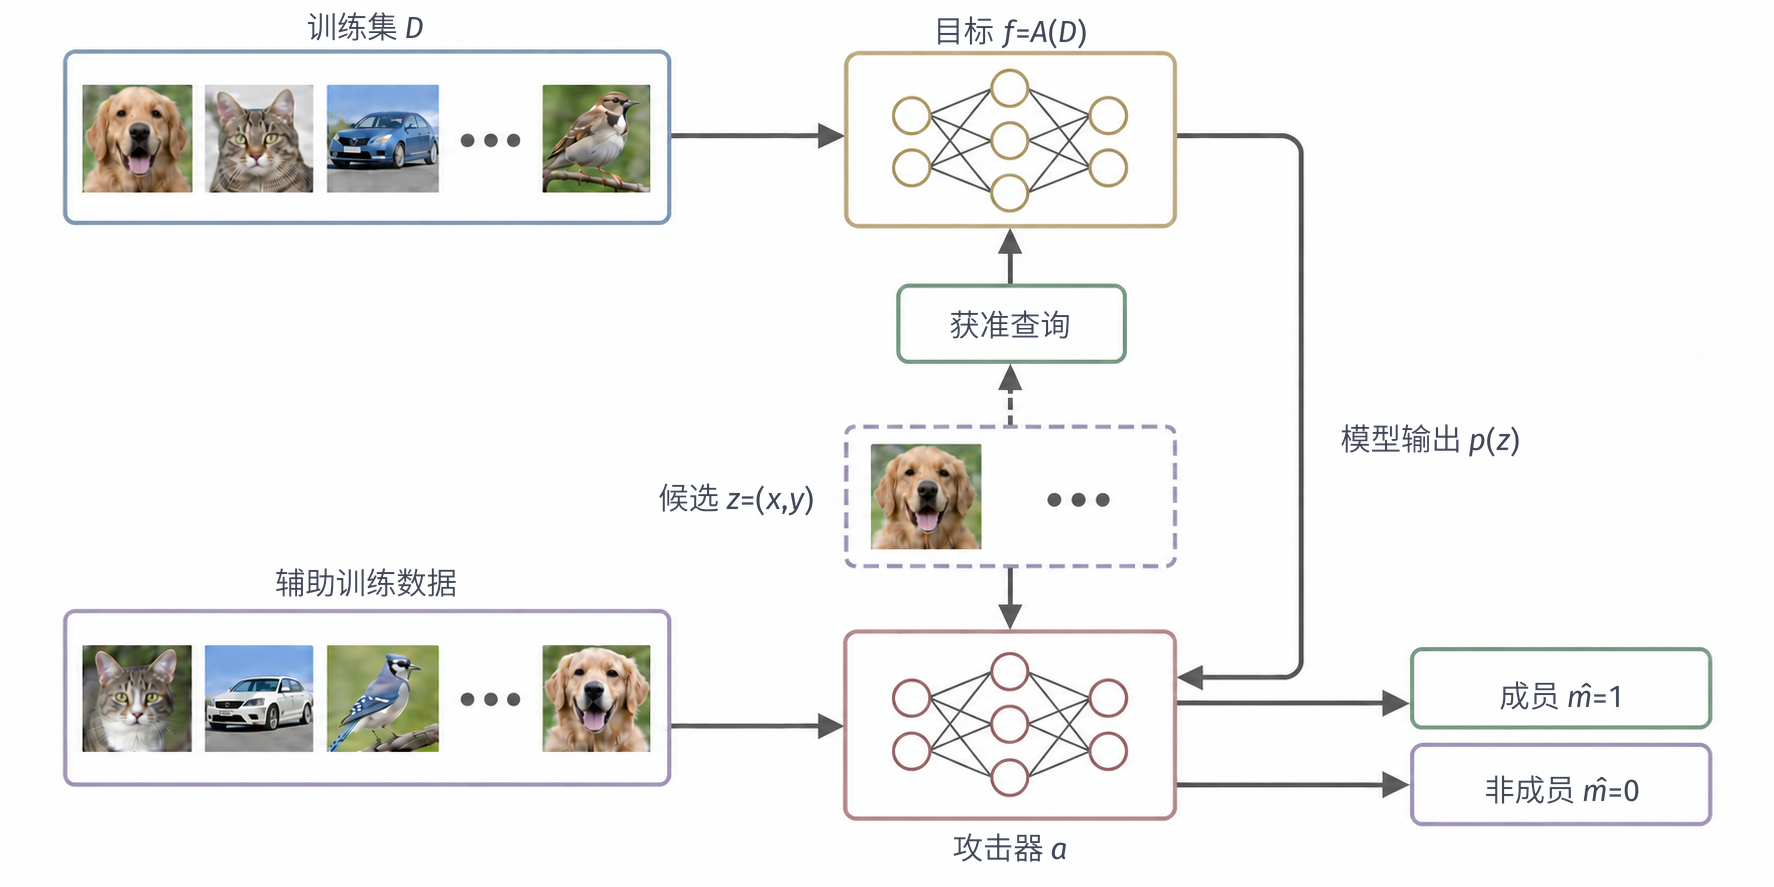
\includegraphics[width=164.600mm]{figures/02-foundations/03-trustworthiness/generated/membership-inference/figure.png}
  \caption{成员推断的受控审计流程。候选成员与非成员按同一分布抽取，目标模型仅用$D$训练；记录$z=(\bm x,y)$经获准查询取得输出。图标个数表示分组，不表示成员先验；已知真实$y$时可以计算损失。攻击器用辅助成员数据训练，在验证数据上定阈值，并在独立审计集统计成员命中率和非成员误报率。目标成员真值用于核验，不能作为攻击器输入。该流程不承诺攻击成功，还须报告权限、查询预算与成员先验。}
  \label{fig:trust-membership-inference}
\end{figure*}

影子模型中的成员差异能否迁移，取决于它是否代表目标训练。数据增强、早停或分布不同，都可能使已学规律失效。总体攻击准确率较低也未必无害：它可能在少数敏感记录上成功。因此，应把平均值与逐记录、逐类别及低假阳性区域的结果一起报告。

Carlini等的\term{似然比攻击}（Likelihood Ratio Attack, LiRA）针对每条待检记录作比较。辅助训练分别估计包含和不包含该记录时的分数分布，再判断目标分数支持哪种假设。该研究用变换后的置信度拟合分布，并强调在很低假阳性率下报告真阳性率\scite{carlini2022lira}。

令记录$z$的观测分数为$s$，包含与不包含它时的密度分别为$p_{\mathrm{in}}(s\mid z)$、$p_{\mathrm{out}}(s\mid z)$。理想检验比较两种解释的相对可能性：
\begin{equation}
 \Lambda_z(s)=
 \frac{p_{\mathrm{in}}(s\mid z)}
      {p_{\mathrm{out}}(s\mid z)}.
 \label{eq:privacy-membership-likelihood}
\end{equation}
分母为正时，上式是普通密度比；分母为零而分子为正时取$+\infty$。两密度都为零的分数集合在两个假设下均为零概率，可任意约定该处比值而不改变检验结果。对完全指定的两个简单假设，似然比在给定假阳性约束下具有最优检验功效，依据是\BookTheoremRef{thm:statistics-neyman-pearson}{第一卷“随机变量”章的Neyman--Pearson定理}。有限辅助训练只能估计密度，经验LiRA因而不能直接继承无条件最优性。逐记录比较旨在区分原有难度与训练参与带来的优势：同是$0.95$预测概率，一封邮件若在两种假设下都容易预测，似然比可能接近1；罕见邮件若只在参加训练时常得到该分数，似然比才可能明显大于1。影子模型提供学习成员规律的一般流程，LiRA在此基础上明确逐记录的双假设比较。

\begin{example}[成员先验改变结果的含义]
\label{ex:privacy-membership-prior}
设候选中真实成员占$1\%$，检验真阳性率为$0.8$、假阳性率为$0.1$。一万条候选预计检出80个真实成员，却同时误报990个非成员；全部阳性中真正的成员约占$7.5\%$。即使检验在成员与非成员各半的数据上结果尚可，实际低先验下的阳性可信度也可能很低。这个教学例子要求报告先验，而不能只移用平衡测试集的表现。
\end{example}

\paragraph{发布模型中的训练数据提取}

知道一封邮件参加训练，只取得了一个二元事实；恢复内容则可能取得整段私人信息。Carlini等以GPT-2研究查询中复现训练序列的情况，区分文本概率高与实际能够提取文本。实验显示发布模型可能暴露训练片段，平均泛化误差不足以概括这种风险\scite{carlini2021extraction}。

生成常见句子未必说明恢复了特定训练内容。受控实验可加入来源唯一的合成标记，再检验复现；真实数据实验则需核来源、去重并与对照语料比较。合成标记便于比较机制，却可能不同于自然记忆；真实内容更接近应用，来源证据不足时又可能混入公开重合或猜测。报告要保留这些证据强度差异。

邮件例子先生成不含真实个人信息的唯一项目编号，仅写入指定训练邮件，并保留无该编号的对照语料。训练后固定提示组、解码规则和一次完整试验的查询预算$k$，保存全部输出并计准确复现次数。随机解码时，以独立种子重复整次试验，用至少提取一次的试验比例估计该预算下的成功率；确定性过程报告实际结果，重复相同输出不增加证据。还需与未训练该邮件的模型或对照训练比较，自适应改提示所花的查询也计入预算。所得结论是指定策略的可提取性，不能穷尽模型内部是否保有信息。遗忘审计可复用同样提示与预算，比较删除前、删除后及重训练参照。

\paragraph{共享更新中的输入重构}

共享更新使审计还需回到训练中途。Zhu等的梯度深度泄露（Deep Leakage from Gradients, DLG）在模型与梯度已知时搜索候选输入和标签，使它们产生相近梯度。结果说明梯度可以携带私人样本信息；恢复程度仍取决于模型、批次和共享梯度等实验条件，不能把它当作天然匿名摘要\scite{zhu2019dlg}。

线性模型提供容易核算的例子。单条记录采用平方损失$\ell=\tfrac12(\bm w^\top\bm x-y)^2$，参数梯度为$(\bm w^\top\bm x-y)\bm x$。残差和梯度非零时，即使不知道残差数值，观察者也得到关于$\bm x$方向的限制；再取得偏置梯度，会增加信息。这个关系只说明没有传原文仍可能传出内容线索，不能证明任意模型都能精确恢复。保护应覆盖实际可见更新，而非仅检查请求是否带原始字段。

重构审计应固定已知模型、更新轮次、批次大小和辅助信息，在受控数据中保留真实输入作参照。恢复结果既要与真值比较，也要与仅凭公开先验的猜测比较。图像外观、文本主题相近和私人字段精确一致，是不同强度的证据。常见结构恢复不足以确认特定记录；少量私人字段准确恢复，也不能因整体误差大而忽略。

\subsection{基于数据流与实现的过程核查}
\label{sec:privacy-implementation-verification}

过程核查将承诺逐项对应到数据流与执行条件。直接访问部分检查采集字段、身份权限、存储副本、日志、检索接口和工具接收者，寻找原文绕过保护的位置。统计保护部分检查发布算法是否具备形式机制所需前提，判断已经允许发布的信息是否满足约束。

可为邮件列处理清单：保存到哪里、谁能读取、经历哪些变换、留下什么中间状态、向外输出什么。配置和实现说明再与受控执行记录对照，验证访问拒绝是否生效、日志有无原文，以及备份和调试接口是否遵循相同限制。流程图给出预定路径，不能单独证明运行程序确实按图执行。

DP实现要依次核对保护单位、敏感度、噪声分布、抽样与组合。敏感度是改变一个保护单位时，按所选距离或范数计算的最大输出变化；标量绝对值、票数向量的$\ell_1$范数、梯度的$\ell_2$范数服务于不同机制。调用加噪函数本身未保证尺度正确。逐记录裁剪却把参数解释为用户级，会漏掉同一用户多条贡献的联合影响。

私有数据还可能参与参数选择、早停、超参数搜索和中间结果发布。这些依赖若不在分析中，最终模型就未必具有所声称保证。检查应覆盖随机数实现、日志及其他渠道；保护某个发布接口的证明不包括系统另外输出的原文。

隐私台账应让人从发布版本还原保证。至少要绑定数据和模型版本、保护单位与邻接、贡献限制、抽样实现、噪声参数、会计方法及版本、目标$\delta$、全部可见发布和累计消耗。旧模型或旧接口仍可观察时，历史输出仍属于联合会计；当前回滚或替换不能抹去这些消耗。

仍以关键词计数核验这条链。若承诺增加或删除一封邮件时满足纯$\epsilon$DP，每封邮件的计数贡献须限定为0或1，噪声按敏感度1校准，并登记同数据上的其他发布。核验沿原始字段、计数规则和随机输出逐步进行，配置中的$\epsilon$只是其中一项。

一封邮件若含关键词一百次，按词频相加就可能贡献100，原敏感度1证明随之失效。按旧尺度加噪后，输出即使显得随机，也没有实现原承诺。单元测试可查贡献截断、噪声尺度和重复发布登记；上界仍需对全部允许输入证明，不能由少量测试替代。第~\ref{sec:privacy-statistical-release}节会推导相应机制。

安全聚合和加密计算对应另一组核验对象：参与者能观察什么、哪些串通被允许、协议依赖什么条件。隐藏计算过程尚未限制公开结果泄露多少。过程保密与统计输出保护需分别留证，再检查组合后的数据流。

\subsection{验证结论与适用边界}
\label{sec:privacy-verification-evidence}

审计结论须与实际比较对象对应。控制来源等混杂因素后，成员判别成功支持参与信息可被利用；内容提取和重构还需证实恢复内容的来源与特异性。它们恢复的信息不同，不能未经论证就当作同等强度的泄露证据。

成功攻击可以反驳过强的保护声明；失败只表明在这项攻击及其资源限制下尚未发现泄露，不能证明所有输出事件都满足DP。理论参数很大而某个攻击成功率低时，二者也不能相互抵消：一个较弱攻击并未说明参数已经无关紧要。

受控攻击还可为参数给出必要下界。固定相邻数据对和检验事件，真实真阳性率$t>\delta$、假阳性率$f>0$时，须有$\epsilon\geq\log((t-\delta)/f)$。实验只取得率的估计，应以真阳性率置信下界和假阳性率置信上界计算，而非把零次误报当作$f=0$。普通成员分类若未实现相邻比较，也不能直接反推DP参数。证据强度由实验与定义的对应决定。

保护的代价也要评价。输出与数据无关的噪声可满足很强限制，却可能无法完成任务。不同群体的样本数和信号强度不同，相同噪声也可能造成不同效用损失；应结合第~\ref{chap:trust-fairness}章按群体检验，并报告成本。

公平审计可把敏感属性读取限定在受限环境，由指定角色计算预定群体指标。训练和线上决策不因此获得权限，对外仅发布所需统计，并检查小群体、交叉查询和重复发布。最小组规模、访问限制和限流可缓解直接暴露，却不能单独保证个体影响上界；后者还需限制每人贡献、保留跨接口查询历史，并以匹配邻接的可组合机制分析联合发布。验收也分两项：公平证据核重要群体的样本是否充分、统计分母是否有效，隐私证据核属性接收者、发布内容和联合观察边界。删除全部属性会丧失测量差异的证据，无限制开放又会增加暴露；两项要求须共同满足。

\section{隐私保护的实现}
\label{sec:privacy-use}

措施沿私人信息进入系统、参与训练和交付结果安排。采集存储限制输入和明文接触者，训练限制数据对参数与中间更新的影响，发布推理限制接收者所得信息，并处理运行中新增的私人上下文。各处保护可组合，其验证对象由前节的数据流与输出承诺确定，不能仅由一处保护推断全程成立。

\subsection{数据采集与存储中的保护}
\label{sec:privacy-collection}

采集之前先问任务是否需要这项信息。省去无关字段会减少保护范围；必要字段须确定用途、访问者和保留时间。不过，即使数据库访问受限，公开一个人数为1群体的精确均值仍能暴露个人值，因此还要分析输出。

最小化需要在具体字段上验证。例如，先检验移除邮件地址和私人编号后，正文特征是否仍能分类，再决定是否收集或长期保存这些字段。只需本地预测时，计算可留在设备，同时检查遥测和日志有无上传原文。省去收集可避免该路径风险，去姓名或改账户代号却不能保证匿名；正文、时间和关联记录仍可能识别人。

必要信息可以按角色限制访问，隔离用途，约定期限，并在传输和存储时加密。加密限制的是无密钥者的读取能力，解密处理方与最终接收者仍可见明文。因此，解密后的用途和输出也需约束，数据库加密不能证明模型不会泄露训练内容。

必须收集个人值、却不应让接收方准确知道它时，可在发送前本地随机化。这样保护的是交给接收方的输入。接收方先持有明文、随后才随机发布，属于另一种信任安排，需要分别说明。

二元\term{随机响应}（randomized response）给私人位加入发送前的随机性。对$x\in\{0,1\}$，以$p=e^\epsilon/(1+e^\epsilon)$的概率发送$x$，否则发送$1-x$。两种输入产生任一消息的概率比至多为$p/(1-p)=e^\epsilon$，故有本地纯DP。设私人位为1的比例为$\mu$、接收位为$Y$，则$\mathbb E[Y]=(1-p)+(2p-1)\mu$。$\epsilon>0$时可用$(\bar Y-(1-p))/(2p-1)$估计$\mu$；$\epsilon$趋近0时分母也趋近0，误差会放大。这个例子把保护强度同样本量和统计精度的代价相连。

\subsection{训练过程中的保护}
\label{sec:privacy-training-influence}

训练要保留群体规律，同时控制单个对象改变发布模型的能力。可限制更新贡献，也可只让私有模型提供受保护的监督标签；二者都须分析相邻数据下的发布分布。选噪声尺度之前，先以指定距离或范数限制最大输出变化，即敏感度。协作方若能看到发布前更新，还需保护这些中间观测。

\paragraph{限制每次更新中的贡献}

多步训练累积各样本的影响。\term{差分隐私随机梯度下降}（differentially private stochastic gradient descent, DP-SGD）先限制单样本梯度，再对聚合更新加噪，使重复更新可以共同纳入隐私分析\scite{abadi2016dp}。

令批次有$b$条样本，梯度为$\bm g_i$，用$c>0$限制其二范数：
\begin{equation}
 \begin{aligned}
 \bar{\bm g}_i
 &=\bm g_i\min\{1,c/\lVert\bm g_i\rVert_2\},\\
 \tilde{\bm g}
 &=\frac{1}{b}\left(\sum_{i=1}^{b}\bar{\bm g}_i+\bm Z\right).
 \end{aligned}
 \label{eq:privacy-dpsgd}
\end{equation}
零梯度仍取零，$\bm Z$为按隐私分析校准的高斯噪声。固定批次中替换一条记录，梯度和的敏感度至多$2c$。增加删除、抽样或用户分组的约定不同，就要重新匹配敏感度与会计。随后以$\tilde{\bm g}$更新，登记各步消耗。

式~\eqref{eq:privacy-dpsgd}的顺序决定分析单位：各样本分别求梯度和裁剪，再求和、加噪并更新。整批相加后裁剪虽也得到有界向量，却改变了机制，不能直接用逐样本抽样分析。即使最后只发布模型，也要查日志和检查点是否另暴露未受保护梯度。

图~\ref{fig:dp-sgd-update}顺次展开一次更新的裁剪、聚合、噪声和参数更新；账本还需累计全部训练步。

\begin{figure*}[htbp]
  \centering
  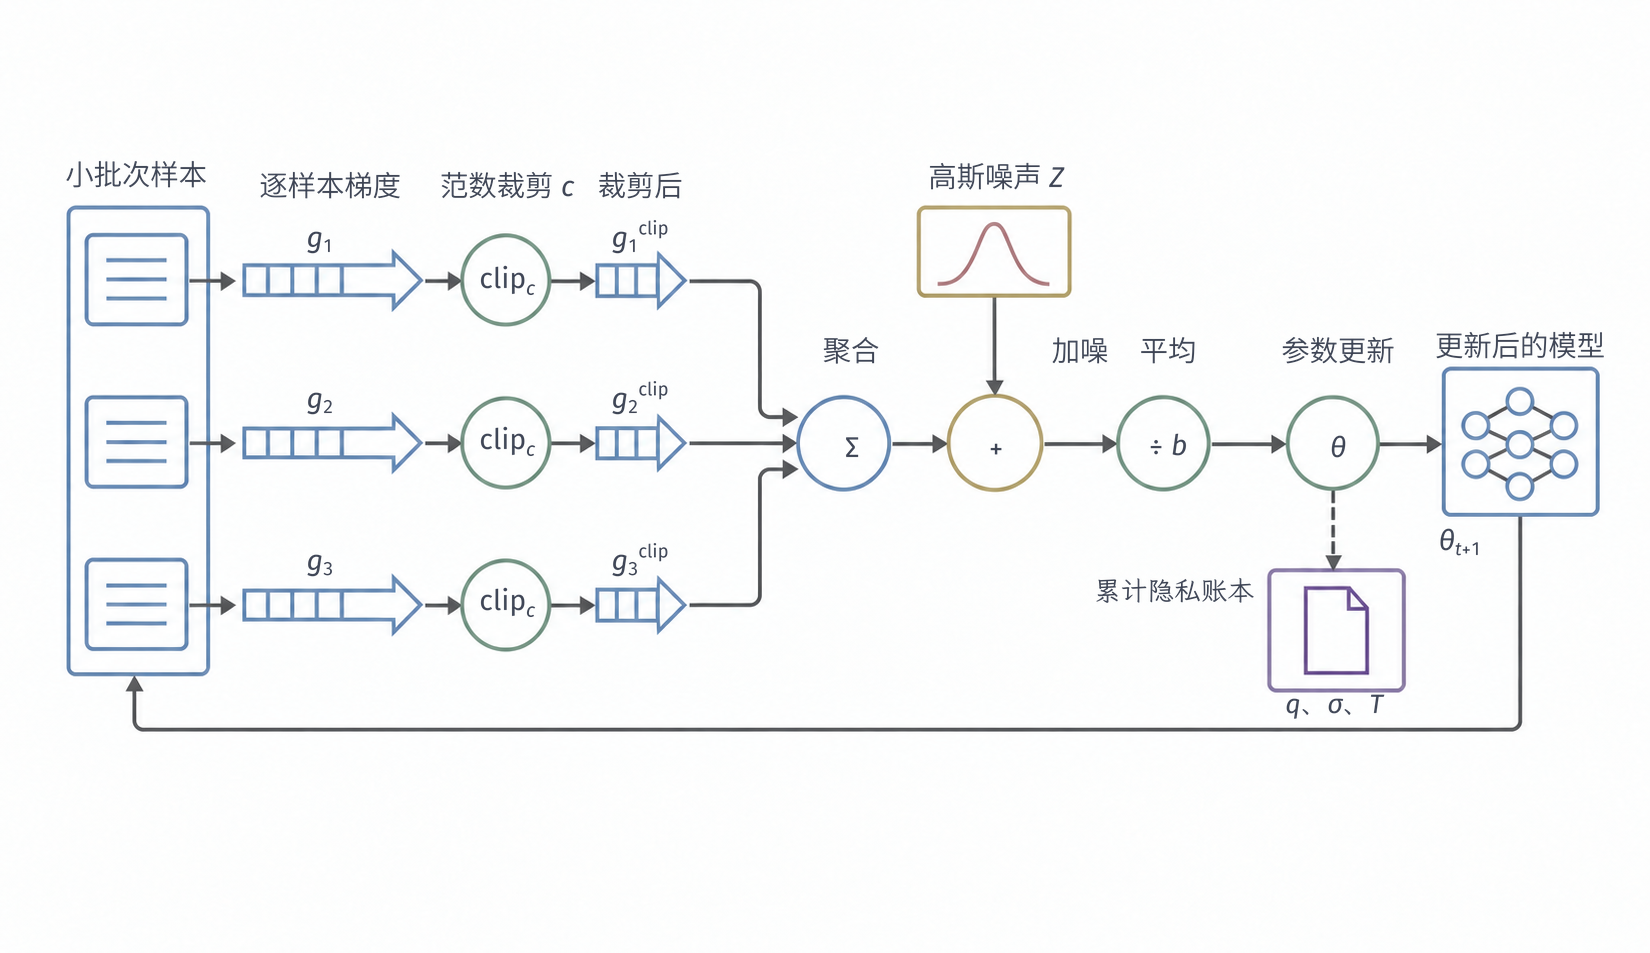
\includegraphics[width=164.600mm]{figures/02-foundations/03-trustworthiness/generated/dp-sgd-update/figure.png}
  \caption{DP-SGD的一次更新。分别计算批次梯度$\bm g_i$，按$c$取$\operatorname{clip}_c(\bm g_i)=\bm g_i\min\{1,c/\lVert\bm g_i\rVert_2\}$，随后求和、加入高斯噪声$\bm Z$、除以$b$并更新。账本结合抽样率$q$、噪声尺度$\sigma$、步数$T$等累计消耗，分析必须对应保护单位、邻接关系和抽样约定。向量长度及高斯曲线只示意机制。}
  \label{fig:dp-sgd-update}
\end{figure*}

裁剪使单样本影响有界，也可能引入偏差；噪声降低更新的可区分性，同时影响优化。预算须结合训练步数、抽样率和噪声强度计算。用户级方案还须控制该用户的总贡献，不能把逐记录裁剪后的多项贡献无限制相加。

噪声可写为$\bm Z\sim\mathcal N(\bm0,\sigma^2c^2\bm I)$，$\sigma$为相对阈值$c$的噪声乘子。独立泊松抽样以概率$q$选各记录，批量大小随机；一种明确机制用数据集大小$n$和期望批量$qn$归一化。改为实际批量归一化或固定大小不放回抽样时，须按实现重写机制，匹配其邻接和抽样会计，不能直接用固定$b$公式。Abadi等以裁剪、噪声和矩会计分析深度训练的重复访问；后续也常用第~\ref{sec:privacy-repeated-use}节的Rényi会计合并更新消耗。

优化与隐私参数要分开比较。固定$q,\sigma,T$（$T$为步数）及邻接约定，改变$c$时按相同比例缩放噪声，通常不改变由噪声尺度与敏感度的比值决定的隐私界。优化轨迹却会变化：小$c$压缩更多梯度，大$c$增加绝对噪声。批量变大也改变平均更新的信噪比、抽样率及完成同轮数所需步数，因此须固定训练预算口径，才能判断隐私有无改善。

公开预训练可帮助保留效用。只要未使用本次保护的数据，会计就从后续私有访问开始；冻结部分参数虽可省计算，其余更新仍需裁剪和完整分析。若用私有数据选模型、构词表或筛样本，这些前置依赖也属于发布算法，不能因在梯度下降之前就不计。

\paragraph{限制监督标签中的私人知识}

若大模型每次更新加噪的损失过高，可让私有模型只回答有限的受保护监督查询。\term{教师集成的私有聚合}（Private Aggregation of Teacher Ensembles, PATE）将敏感数据划为互不重叠分区，教师各用一片训练；学生以非敏感输入查询，再用带噪投票标签学习。保护接口是聚合，教师自身不发布\scite{papernot2017pate}。

记第$j$类票数为$v_j(\bm x)$，一种聚合返回$\arg\max_j\{v_j(\bm x)+Z_j\}$。固定分区规则，一条记录至多改变一个教师的票；从一类移到另一类，票数向量的$\ell_1$变化至多2。该界来自数据隔离，并不要求教师优化凸性。一个用户跨多个分区时，可改变多位教师，必须重算用户级影响。

共识高时，一票通常难以改变答案；近乎平票时则更容易改变。可扩展PATE采用高斯聚合，以带噪共识阈值决定是否回答，用投票差距细化隐私会计。回答与否也依赖私人数据，该门控同样需要计入消耗\scite{papernot2018pate}。

拒绝低共识查询也会筛选学生的训练数据。罕见邮件可能更难获得共识，应按群体检查标签获得比例与学生效用；这个比例不同于预测集合覆盖率。实际顺序是先训练保持私有的教师，再为来源明确的非敏感输入查询带噪标签，最后训练学生，每次新查询都计入访问。PATE把接口放在监督标签上，教师可用不同内部算法，却需要适合学生的非敏感输入，并受查询数和共识不足限制。DP-SGD直接控制私有更新，不需教师分片或这种输入。比较两者须先统一保护单位，最终噪声数值不能单独代表保护强弱。

学生若只使用公开输入、受保护标签和独立随机性，给定这些标签后便与私人数据条件独立，可以应用后处理性质。继续读取教师、原始记录或其他数据依赖状态，就会新增需要会计的访问；将学生放回私人数据训练也属于这种情况。

图~\ref{fig:pate-private-teachers}示意教师与学生之间的边界。公开查询输入取得受保护聚合标签用于学生学习，私有样本没有直接交给学生。

\begin{figure*}[htbp]
  \centering
  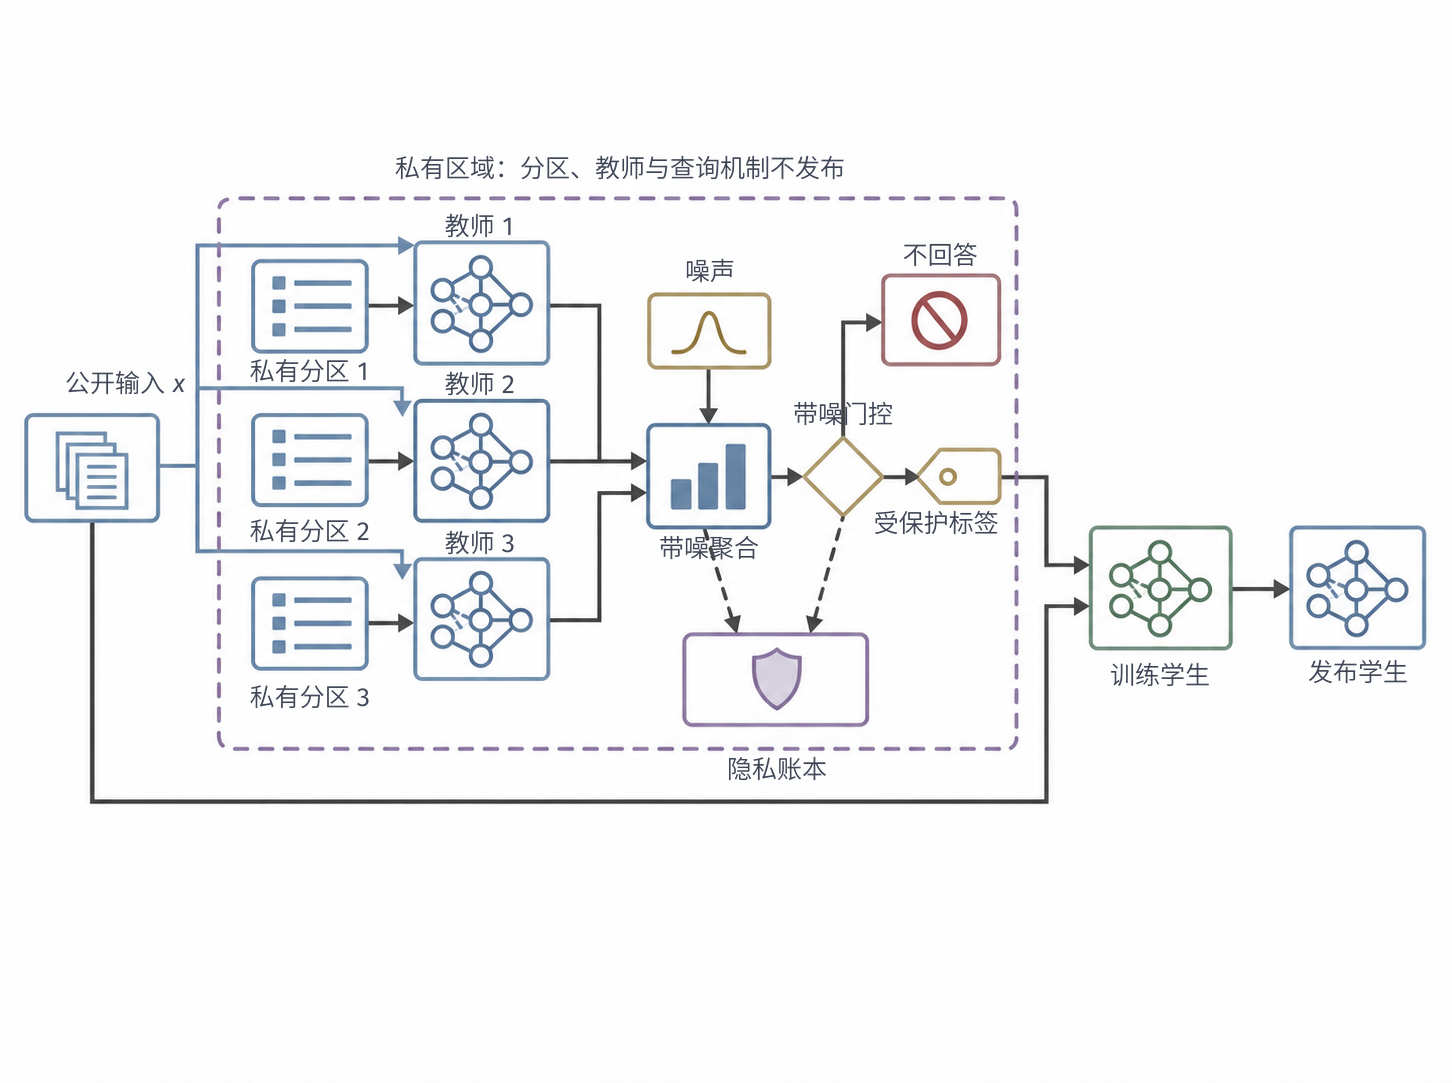
\includegraphics[width=164.600mm]{figures/02-foundations/03-trustworthiness/generated/pate-private-teachers/figure.png}
  \caption{PATE的信息流。各教师用互不重叠的私有分区训练并保持不发布，非敏感公开输入取得各教师投票。加噪聚合和带噪门控产生受保护标签，低共识可不回答；两项决定均计入查询隐私消耗。学生仅以公开输入和受保护标签训练后发布，不能接触私有样本或单个教师。蓝线为公开查询，灰线为训练与投票，虚线为隐私记账；条形表示投票机制，不是实测数值。}
  \label{fig:pate-private-teachers}
\end{figure*}

\paragraph{协作方可见的中间更新}
\label{sec:privacy-collaborative-computation}

最终发布的保护尚未处理参与者可见的训练更新。服务器和其他客户端可能在发布前取得这些观测，所以要先列明各方权限与允许串通的范围，再决定怎样隐藏中间信息。

安全聚合（secure aggregation）把服务方的可见结果限制为多个参与者的聚合；安全多方计算（secure multi-party computation, MPC）和同态加密（homomorphic encryption, HE）在受限的中间可见信息下完成指定计算；可信执行环境（trusted execution environment, TEE）则以隔离执行和硬件假设为依据。它们解决计算过程的保密问题，若最终模型仍保有私人内容，还须分析输出泄露。

Bonawitz等针对客户端向服务器提交向量并求和设计安全聚合协议。客户端更新先带掩码发送，聚合时掩码抵消，协议另处理部分客户端退出后的恢复。论文按对手与串通条件分析服务器可得总和而不可得单项更新的范围\scite{bonawitz2017secureaggregation}。

总和本身也可能泄露。其余贡献已知而仅剩一名未知参与者时，观察者可从总和确定该人的贡献；多轮高度重合人群的统计，也可能通过作差提供线索。因此，参与人数、串通阈值与发布规则须和安全聚合一起说明。分布式加噪还需证明噪声由谁产生、多少诚实参与者留存，以及退出后总噪声是否仍足够。

图~\ref{fig:federated-learning-process}将本地记录、上传更新和中心聚合区分开。记录虽留在设备，更新仍是由私人数据产生的观测，须按上述权限与串通条件检查。

联邦学习将计算移到数据所在位置，本身不提供这些隐私条件。本地记录级DP-SGD与裁剪客户端总更新的用户级方案，保护的单位不同。信任中心时可在安全聚合总和上由服务器加噪；不信任中心时，需要客户端共同提供足量噪声或采用其他信任安排。通信加密、聚合保密和统计输出保护应连接到同一数据流，分别实现各自承诺。

\subsection{结果发布与推理使用中的保护}
\label{sec:privacy-statistical-release}

开放权重、限制查询和发布统计表，给接收者的观察能力不同。发布前应逐项确认实际可见内容：减少无关分数、原始字段和调试信息，可收窄直接暴露；限接口和查询数，可减少某些攻击的观测。要宣称DP，仍需针对相应机制分析，不能由这些操作限制单独推出。

\paragraph{发布统计量中的个体影响}

可信管理者已拿到明文后，还要控制公开统计量对个人的暴露。小群体精确统计或反复差分查询，即使不含原文，也可能确定个人值。下面以统计量的发布分布作为保护对象。

设要发布实值统计$F(D)$。在给定相邻关系下取$\Delta F=\sup_{D\sim D'}|F(D)-F(D')|$，限制一个保护单位能够造成的最大变化，再据此选择噪声：
\begin{equation}
 M(D)=F(D)+Z,\qquad
 Z\sim\operatorname{Laplace}(0,\Delta F/\epsilon),
 \label{eq:privacy-laplace}
\end{equation}
这里要求$\epsilon>0$及$0<\Delta F<\infty$。敏感度为零时，统计量对相邻变化不变，无需为此加噪；敏感度无界时，则须先限定数据域或贡献，或另选机制，不能使用一个有限拉普拉斯尺度。

式~\eqref{eq:privacy-laplace}为何具有纯$\epsilon$DP，可以直接比较同一输出位置$u$的密度：
\[
 \exp\left(
 \frac{|u-F(D')|-|u-F(D)|}{\Delta F/\epsilon}
 \right)\leq e^\epsilon,
\]
三角不等式把分子差限制为敏感度，对任意输出事件积分，就得到式~\eqref{eq:privacy-definition}的$\delta=0$情形。噪声尺度由此同最大数据影响相连，不能先任意加噪再为它命名隐私参数。

图~\ref{fig:trust-dp-neighbors}以相差一条记录的计数比较随机发布。上部将准确值与同分布噪声相加，下部展示所得分布。观察者只取得一次随机输出，定义限制的是两种数据下所有事件的概率关系，并不要求两次可能输出取同一数值。

\begin{figure*}[!htb]
  \centering
  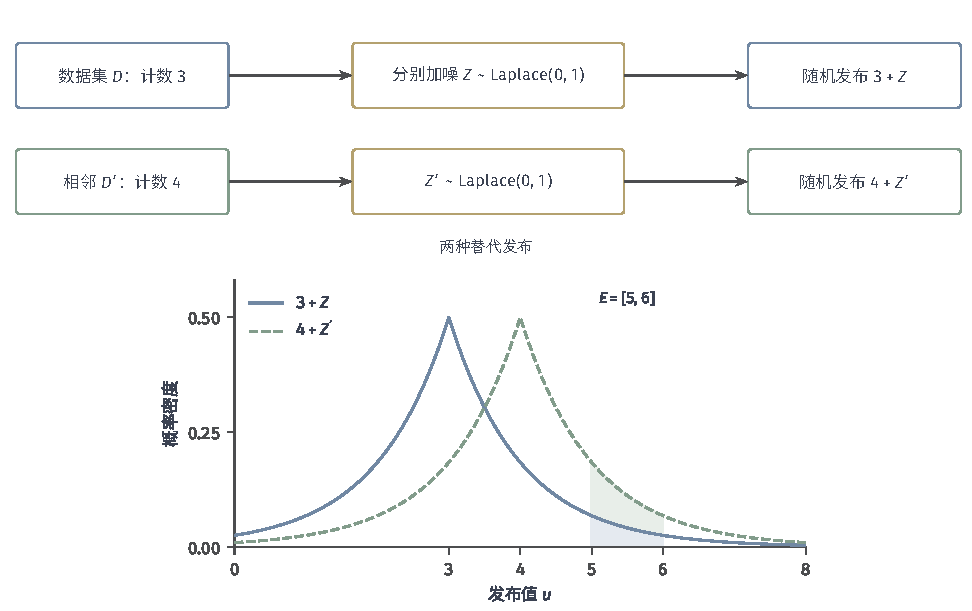
\includegraphics[width=164.600mm]{figures/02-foundations/03-trustworthiness/matplotlib/trust-dp-neighbors-comparison/figure.pdf}
  \caption{相邻计数的随机发布。两数据集仅差新增一条记录，准确计数为3和4；各反事实机制都使用尺度1的拉普拉斯分布，故$\Delta F=1$、$\epsilon=1$、$\delta=0$。两行是替代发布情形，不表示共同发布两次，也未规定联合耦合。每一行由准确计数经加噪得到随机发布，下方实线与虚线为解析密度，阴影比较同一事件$E=[5,6]$；横轴只画部分范围。一次输出的保护须对全部相邻数据和全部事件成立，曲线重叠只是示意。}
  \label{fig:trust-dp-neighbors}
\end{figure*}

关键词邮件数每条贡献至多1，记录级敏感度为1。取$\epsilon=0.5$时，加入尺度2的Laplace噪声；相差1的两计数会产生重叠输出，不能再由一个准确整数确定目标邮件是否存在。若保护一名用户且每人最多贡献10封相关邮件，敏感度变为10，同$\epsilon$要求尺度20，除非另限制贡献。这个代入例子把保护单位、噪声和效用代价对应起来。

\begin{example}[计数与平均值的不同要求]
\label{ex:privacy-sensitivity}
增加删除相邻下，人数计数的敏感度为1。均值则需要另一组条件：固定$n$条记录，按替换一条定义相邻，数值预先限于$[0,1]$，敏感度才为$1/n$。取消值域限制可能使它无界。两例的邻接约定不同，不能仅凭都叫统计量便使用同一尺度。
\end{example}

\paragraph{推理上下文与结果接收者}
\label{sec:privacy-inference-context}

推理新增的信息流也要逐处限制。检索私人文档、调用工具或保存对话日志，会把敏感内容送入新的接口。应提供必要上下文、限制工具字段，并确认输出内容及接收者。若这类输入也承诺形式保护，其新访问必须纳入所用机制分析。

这里保护当前请求的私人信息，范围已超出训练记录。模型即使满足训练数据DP，收到新邮件后直接转交外部工具，仍可能泄露请求。上下文进入模型、字段进入工具和结果交给接收者，都需要各自的信息边界；训练保证不能自动覆盖新增输入。

权限控制可在检索前实施，只把用户有权查看的文档送入上下文。随后工具仅获任务必要字段，回复与工具请求核接收范围，日志限制保存内容。输出过滤可拦已知标识或模式，却会遗漏改写和间接推断，也可能误删合法内容，需分别用结果检验和过程核查确认。过滤测试有效仍不足以宣称上下文形式隐私成立。

\paragraph{多次发布的累计保护强度}
\label{sec:privacy-repeated-use}

已有发布$M(D)$之后，若随机映射$K$给定该结果便与$D$条件独立，即仅使用$M(D)$、公开信息和独立随机性，$K(M(D))$就不增加DP参数。后处理事件可转写为原输出上的随机检验，继续受式~\eqref{eq:privacy-definition}限制，这就是后处理性质。若另读由$D$生成、却未纳入$M(D)$发布保证的额外缓存、模型或统计量，就会新增数据依赖，不能应用这项纯后处理结论。

重新读取数据运行机制，需要组合保护。基本界将各步$\epsilon,\delta$分别相加；自适应时，每步给定先前输出仍须对同一邻接满足所声称的条件界。利用结构可得到更紧会计，但重复试验和模型选择仍须纳入。查询已发布私有模型而不新增数据访问，与每次重新读取私人上下文，属于不同过程。

同一保护对象影响多个发布时，观察者可以联合利用它们，预算也必须累计。以下组合用于训练更新和持续服务，可跨采集、训练、发布阶段使用，并不是另一个处理阶段。

同批邮件以$\epsilon=0.5$计数，重新抽噪发布三次，基本组合得到纯DP上界1.5。只把已发布的一次计数画图、换单位或再显示，则是后处理，不新增该预算。调用分属不同网页或功能，也不能拆开忽略同一对象的访问；会计应覆盖观察者联合可见的结果。

训练更新常达数千次，每步都转成$(\epsilon,\delta)$再求和可能过松。\BookDefinitionRef{def:information-renyi-divergence}{第一卷“信息论与统计几何”章的“Rényi散度”定义}与\BookSectionRef{sec:information-sequential-accumulation}{同章的“序列信息累积”一节}已给出散度及逐历史统一条件下的自适应组合；这里把这些工具用于隐私邻接。\term{Rényi差分隐私}（Rényi differential privacy, RDP）要求所有相邻数据的输出分布在相应阶数下具有统一散度上界。对$P,Q$及$\alpha>1$，沿卷一记号写为
\begin{equation}
 D_\alpha(P\|Q)=\frac{1}{\alpha-1}
 \log\mathbb E_{o\sim Q}
 \left[\left(\frac{\mathrm dP}{\mathrm dQ}(o)\right)^\alpha\right].
 \label{eq:privacy-renyi}
\end{equation}
相邻输出间该量均不大于$\rho(\alpha)$时，便得到这一阶RDP。绝对连续和无穷值约定同卷一。Mironov建立此定义及组合、后处理和转换性质\scite{mironov2017rdp}。

第$t$步若给定任意此前输出仍有统一的$\rho_t(\alpha)$界，组合得到$\sum_t\rho_t(\alpha)$。事先指定$\delta\in(0,1)$后，可转换为
\begin{equation}
 \epsilon(\delta)=
 \inf_{\alpha>1}\left\{
 \sum_{t=1}^{T}\rho_t(\alpha)
 +\frac{\log(1/\delta)}{\alpha-1}
 \right\}.
 \label{eq:privacy-accounting}
\end{equation}
取下确界只在已证明有效的阶数界中选择，不再读取私有数据。不含抽样的高斯发布有$\rho(\alpha)=\alpha\Delta_2^2/(2s^2)$，$\Delta_2$为向量统计的二范数敏感度，$s$为逐坐标噪声标准差。抽样会改变曲线，不能简单把抽样率乘到最终$\epsilon$；独立泊松和固定大小不放回需不同放大分析。选择样本若依赖私人数据，也不能沿用数据独立抽样的放大结论。

\section{数据撤回与模型消除}
\label{sec:privacy-unlearning}

邮件撤回后，我们希望移除的是这些指定记录的训练影响，称为\term{机器遗忘}（machine unlearning）。本节“模型消除”指这一目标，并非删除或停用整个模型。清除文件、阻止文本输出和消除训练影响，各有自己的验收对象。

用$A$表示训练算法、$D$表示原数据、$F$表示撤回记录、$U$表示模型更新程序。图~\ref{fig:trust-privacy-deletion}区分保留数据与模型更新：数据清理并不改写旧模型，更新后的影响则要同从未使用$F$的重训练比较。一个提取测试没有恢复私人片段，只支持该测试结果，尚未说明全部训练影响消失。

\begin{figure*}[htbp]
  \centering
  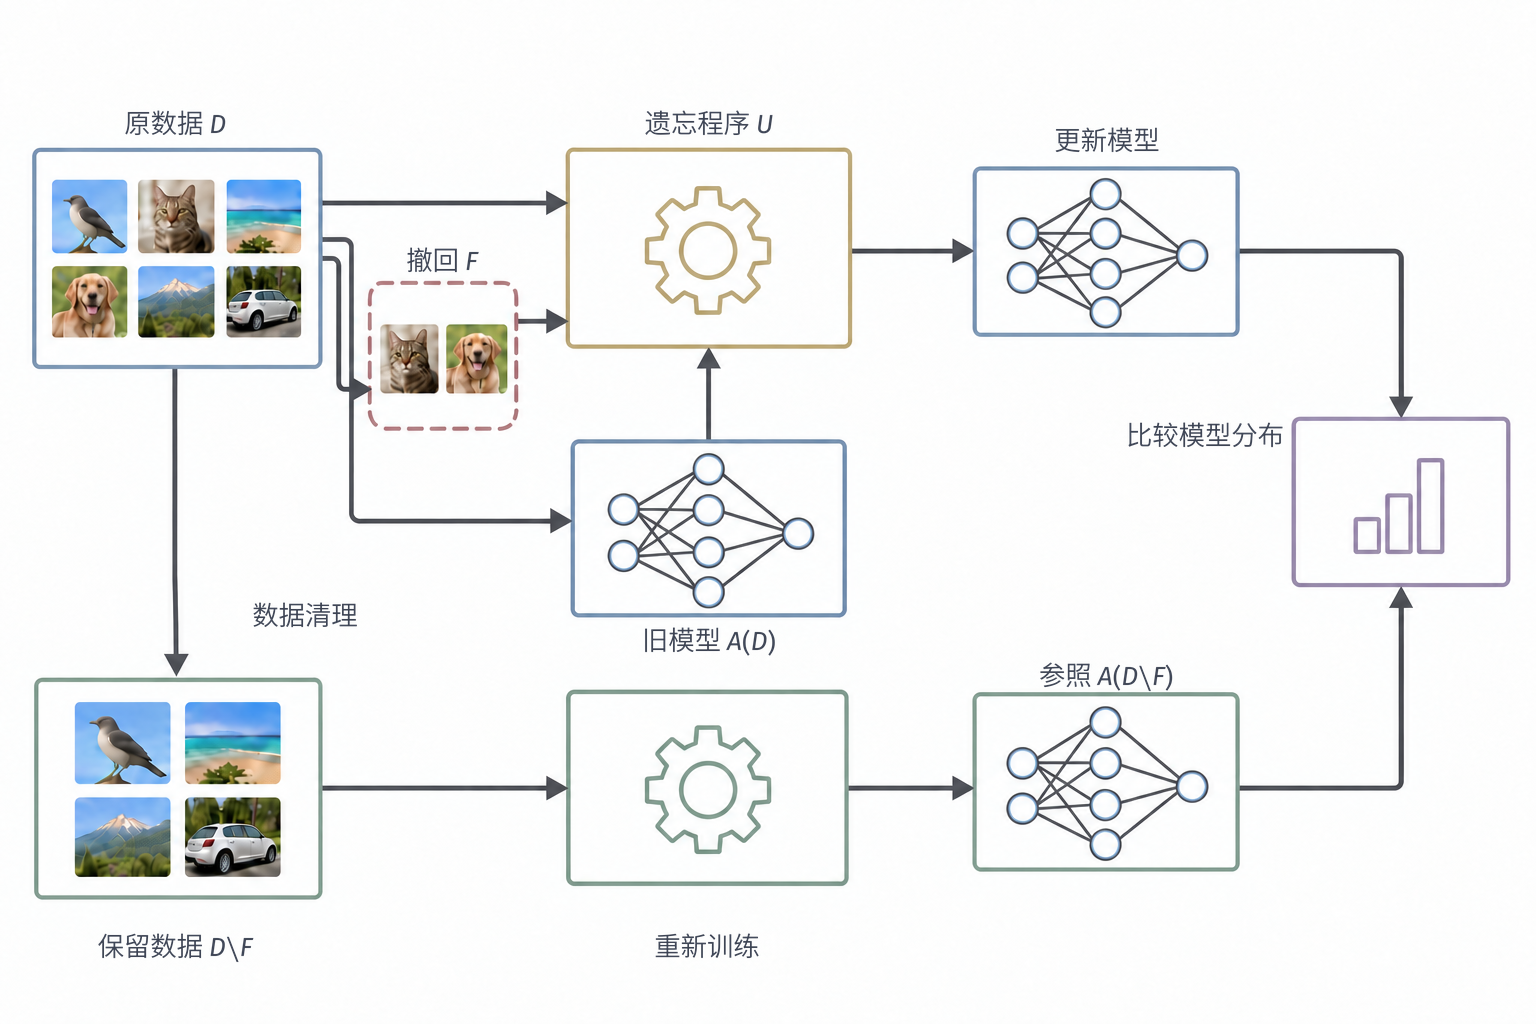
\includegraphics[width=164.600mm]{figures/02-foundations/03-trustworthiness/generated/unlearning-reference/figure.png}
  \caption{数据清理与训练影响消除。删除记录得到$D\setminus F$，旧模型$A(D)$仍保持原状态；$U$另外读取旧模型、原数据和撤回集合进行更新。应比较更新结果与从未使用$F$的重训练模型分布：精确遗忘要求同分布，近似遗忘需指定距离或可区分性标准。}
  \label{fig:trust-privacy-deletion}
\end{figure*}

集合差先按记录身份定义，并限定观察者只取得替换后的新发布模型，不再持有旧模型、旧回复、日志或辅助状态。在这一视图内，精确遗忘要求
\begin{equation}
 U(A(D),D,F)\ \overset{\mathrm d}{=}\ A(D\setminus F).
 \label{eq:privacy-exact-unlearning}
\end{equation}
$\overset{\mathrm d}{=}$比较训练与遗忘随机性产生的已发布模型分布，并非一个固定模型对某个请求的预测分布\scite{bourtoule2021sisa,guo2020certifiedremoval}。右侧由从未使用撤回记录的训练得到。观察者若还能联合读取旧模型、回答或其他状态，就要比较联合观察分布；新模型边缘同分布不能收回已披露的信息。程序可保存额外状态，但可见状态同样须纳入参照。

近似遗忘把同分布放宽为在指定距离或可区分性标准下接近。也可以另定义参数、预测或攻击结果的比较，但行为与攻击只考察模型经过特定观察映射后的量。少量请求上结果接近，除非另有证明，不能推出整个发布模型分布接近重训练。

DP与遗忘各自比较不同对象。DP训练限制参与对输出的影响，遗忘在撤回后比较指定记录删除时的重训练。二者可配合，使用DP却不能单独证明任意撤回要求已经完成。

一次撤回首先要确定范围，停用相关数据，清理可控制的副本和衍生状态，并隔离尚不能清除的部分。这些是每项请求都要做的工作。数据已进入训练结果时，再在完整重训练、局部重算和参数修正中选择满足遗忘标准的方案；三者互为备选，无需依次执行。正式处置完成前的输出限制属于过渡措施。最后分别验收资产、接口和模型影响，同时计完整流程的时间与资源。

\subsection{撤回范围与数据资产清理}
\label{sec:privacy-asset-deletion}

定位时利用稳定记录标识、用户关联和计算依赖，找到原始文件、清洗副本、特征缓存、检索索引、向量记录、训练快照及相关日志。用户级撤回不能止于账户表的一行；记录同时涉及多人时，还要指定删除整条还是其中字段。范围确定后，后续处置才有可核对清单。

快速响应依赖事先保存的数据去向。记录与数据版本、索引项、训练任务、模型版本之间的映射，可用于生成撤回任务。确认请求后，先阻止数据再入训练队列、检索和新副本，随后按存储依赖清单删除或重建，并核正在运行任务有无旧快照。删除标记可以停止正常使用，物理副本真正清除则是另一个完成状态。

模型修正可能还要读撤回记录，所以清理顺序需与更新协调。贡献扣除需其统计量，部分参数修正需其损失；若必须读取原文，可在受限撤回环境完成，再删除工作副本。已有统计状态够用时可免读取，但状态本身也须核私人信息。停止正常训练和检索，不意味着立即销毁算法尚需的一切输入；临时副本的权限、存续期与最终清除仍属本次验收。

删除索引还需处理衍生缓存。文档移除后，向量、片段缓存和生成摘要可能继续被检索或复用；备份恢复时也应重新执行撤回记录，防止旧数据回流。无法立即逐条清理的归档，要明确隔离、清除计划及恢复限制。在线不可见只能描述当前接口，不能表述为所有副本已消失。

按存储和依赖清单验收，逐项区分完成、待处理和无法控制的副本，测试记录能否继续被检索、导出或训练，并绑定模型版本。审计日志需证明处置过程，也应避免再次保存完整私人内容。资产清理解决仍保存和再使用的问题，参数里的训练影响还须进入下一节的方案选择。

\subsection{训练影响的消除方案}
\label{sec:privacy-unlearning-methods}

已经参与训练的记录，需要按遗忘标准、算法结构和可用状态选择消除方案。完整重训练直接生成参照，局部重算依赖可追踪计算，参数修正则从旧模型出发，近似求得删除后的结果。三者条件与证据不同；耗时少只说明计算节省，不能单独代表遗忘充分。

\paragraph{完整重训练}

完整重训练在$D\setminus F$上重新运行$A$，直接生成式~\eqref{eq:privacy-exact-unlearning}右侧的参照，代价是再处理保留数据和训练模型。它比较同一流程下的模型分布，不要求一组随机参数恰好重现。

参照还包括用$F$完成的前置处理。词表、标准化、样本筛选和模型选择若依赖撤回记录，就须重算；受$F$影响的优化器状态或初始化检查点，也不能直接作为从未读过$F$的起点。公开预训练或中间结果只有确定独立于$F$时才可复用。早停轮数、随机抽样及其他训练规则都属于$A$，需要一起固定。

新模型完成后，还要切换服务、使旧缓存失效，记录覆盖的撤回请求。合并多项请求可以省去重复训练，等待期间却仍须限制旧数据和服务暴露，报告实际等待时长。进入批处理队列只是安排，不能据此把模型影响标为已消除。

\paragraph{局部重算}

要减少重训练工作量，先确定记录影响哪些计算。模型若只依赖可更新统计，可扣除该记录的贡献；训练若事先隔离为多个部分，可只重算受影响的部分。两种节省均依赖已知计算结构，并不意味着任意网络参数中都能找到一条记录的位置。

Cao和Yang将学习过程组织成可更新的求和形式，撤回时修改对应统计，减少对保留数据的重复处理。算法和前置处理须确实符合这一结构，并能追踪衍生数据依赖，才可采用贡献扣除\scite{cao2015unlearning}。

考虑仅用记录数$n$和数值和$S$计算$\hat\mu=S/n$的教学估计器。撤回$m<n$条记录，令其和为$S_F$，可直接更新
\[
 \hat\mu_- =\frac{S-S_F}{n-m}.
\]
数学上等同于重新对保留数据求均值，只需知道撤回贡献；实现仍有浮点误差。对$1,2,3$删除3，更新得$(6-3)/(3-1)=1.5$。这证明特定统计模型可以精确扣除，却不能推为深度训练中减回某个梯度即可：后续步骤依赖先前参数，也受该记录连带影响。

另一种结构在训练前隔离依赖。SISA按分片、隔离、切片与聚合（Sharded, Isolated, Sliced, and Aggregated）组织训练：分片各自训练子模型，内部依序处理切片并保存检查点，最后聚合预测。删除记录时恢复到它首次进入之前的状态，再重算相关后续步骤。局部节省由预先隔离获得\scite{bourtoule2021sisa}。

例如，邮件预先分四片，每片含三个顺序切片，待删除记录在第二分片的第二切片。其他三子模型可保留，第二分片从第一切片末状态开始，在排除该记录后重算后两个切片。节省来自依赖隔离，而非从最终参数任意抽出记录影响。全数据上的标准化、词表和模型选择若仍共同计算，就会形成跨片依赖，必须一起处理。

分片增多会减少各子模型数据，也可能改变集成相对整批训练的效用；检查点越密集会增加存储和敏感状态管理成本。因此，评估不能只计一次删除时间，还要计初训、保存状态、常见请求分布和保留任务效用。给定删除条数时，应检验使受影响分片数或重算时间最大的请求位置，并固定所比较的重训练算法。

SISA更新的参照应采用同样分片、切片和聚合规则，还要核删除后抽样与随机状态的处理。整批单模型本来是另一训练算法，不能用与它的比较宣称SISA输出分布相同。

\paragraph{参数修正与近似遗忘}

依赖没有事先隔离时，可从当前参数出发，近似求得删除后的模型。参数改变量小，并不能直接说明指定记录的影响已被充分消除；需要另给误差和分布依据。

Guo等的认证删除为一类正则化线性模型控制近似误差：牛顿更新逼近删除后的解，训练目标中的随机扰动再遮掩剩余误差。强凸性、平滑性等条件共同支撑保证，仅有小梯度残差还不足以证明删除成功\scite{guo2020certifiedremoval}。

先看更新的优化作用。原参数为$\hat{\bm\theta}$，删除后的光滑强凸目标为$L_-(\bm\theta)$；在原参数处，梯度与海森矩阵为$\bm g_-,\bm H_-$，一步牛顿近似为
\begin{equation}
 \tilde{\bm\theta}
 =\hat{\bm\theta}-\bm H_-^{-1}\bm g_-.
 \label{eq:privacy-newton-removal}
\end{equation}
目标局部近似二次时，此步可去除主要一阶偏差，剩余误差可由$\lVert\nabla L_-(\tilde{\bm\theta})\rVert_2$刻画。确定性误差再小，观察者仍可能利用精细参数差别识别记录。因此，认证还需把残差与随机扰动的分布连起来，证明输出按既定可区分性标准接近重训练。

对无约束可微强凸目标，设强凸参数为$\lambda>0$，最优解为$\bm\theta_-^*$，则$\lVert\tilde{\bm\theta}-\bm\theta_-^*\rVert_2\leq\lVert\nabla L_-(\tilde{\bm\theta})\rVert_2/\lambda$。这是残差控制参数误差的结论，强度尚不到输出分布隐私界。连续撤回需累计残差与认证预算，超出允许条件时可通过重训练恢复承诺。非凸大型语言模型不具备上述前提，不能直接使用强凸线性分析。

没有认证条件时，深度模型可尝试经验修正。在撤回样本上提高预测损失以压低相应答案概率，同时在保留数据上降低任务损失或约束预测变化。前项减少目标行为，后项限制附带损伤；若仅提高撤回损失，模型也可能靠破坏广泛能力达成。撤回准确率下降因此不是遗忘充分程度的单一指标。

负偏好优化（Negative Preference Optimization, NPO）针对语言模型遗忘更新的不稳定性，以原模型作参考，按目标序列在当前与参考模型中的相对概率调节更新。目标已被明显压低时，权重随之下降；结合保留数据损失，可以限制效用下降。它给出经验参数修正路径，尚未自动保证任意语言模型的参数分布接近完整重训练\scite{zhang2024npo}。

第~\ref{sec:interpretability-local-training}节的局部影响近似可用于估计修正方向，但大规模删除通常超出线性近似范围。数据归因解释样本如何影响行为，遗忘则要求改后模型满足重训练参照标准；方向估计正确，仍不足以提供后者的误差和分布界。多次删除也需核近似误差累积。

方案选择先固定遗忘标准，再比较满足它的响应代价。完整重训适用面广但成本高；统计贡献和隔离训练利用结构省重算；参数修正分别需要认证前提或经验边界。近似结果达不到标准时，应重训或收紧服务范围。最快只是一项成本结论，不能直接命名为最优遗忘。

\subsection{撤回完成前的过渡保护}
\label{sec:privacy-unlearning-output-control}

清理和更新未完成时，可先限制可控接口的暴露。撤下检索文档、失效缓存、减少敏感请求字段、拒绝无权接收者，或屏蔽回复中的已知私人标识，都直接限制服务返回内容。这些可先作为撤回响应实施，再等待完整处置。

最终文本过滤编号并未改参数，改写编号、关联提问、其他接口和旧权重仍可能绕开规则。拒答微调虽改参数，也可能只让模型避开某类问题；拒答增加不能单独证明训练影响消失。知识编辑改变一个答案后，同样要有额外证据，才能宣称指定数据的影响已接近重训练参照。

检索源删除与输出过滤也要分别验收。内容只在外部库时，清记录、索引和缓存可切断该来源；模型若也用这些内容训练，切断检索就仍留下参数问题。数据去向决定是否需要训练影响消除，不能对全部请求套用一种操作。

可先执行输出限制，随后完成影响消除，分别报告各自状态、接口和验收结果。本地更新不会自动删除已经交给外部的内容或模型副本，因此承诺范围只能包括明确可控制的状态和服务。

\subsection{撤回结果与效率的验收}
\label{sec:privacy-unlearning-validation}

验收分三项：清单内副本已删除或隔离，指定接口的临时限制已生效，模型影响已达选定标准。若记录从未进入训练，最后一项可记不适用，但需留数据流和版本证据。资产和模型任一遗漏都会让撤回未完成：例如文件已删仍用受影响旧模型，或模型已更新却又把旧样本送入下一轮训练。

模型项须回到式~\eqref{eq:privacy-exact-unlearning}的参照，不能由重算量或参数幅度判断。受控比较固定$F$、剩余数据和训练规则，保留原模型、遗忘模型与用$D\setminus F$重训的模型，同时核待消除信息与保留任务。

要经验比较式~\eqref{eq:privacy-exact-unlearning}的模型分布，须独立重复训练和遗忘，报告实例数与估计误差。有限样本只支持选定统计或可区分性的估计，精确同分布仍须形式证明。固定模型反复生成，只估给定请求与解码规则的行为分布，并不是新训练实例。两类模型分布证据都缺少时，只能报告行为层结论。

行为评价也要预定设置。每个设置内，三模型使用相同请求、解码和攻击预算；再跨设置改变提示、采样和预算做压力测试，分别报告。项目编号邮件可比较提取与成员分数，并在保留邮件上测分类风险、概率校准和群体表现。随机生成在设置内用独立种子重复，给次数与估计误差，避免将一次随机输出或表层拒答作为完整证据。

不再复现私人项目名原句，只通过了精确匹配检查；改写提示、关联事实和多轮问答仍可能暴露相同信息。反之，不使用该邮件重训的模型也可能从保留邮件学到项目名。要求它完全不能回答该知识，就比移除指定记录影响更强，需要重新定义参照数据和知识范围；否则会把重训本来可知的事实错判为遗忘失败。

遗忘成员审计要调整参照。原成员、普通非成员和撤回记录不构成原样的二类比较；将撤回记录过度排斥、损失抬得异常高，反而可能暴露它曾被撤回。应在遗忘与重训练模型上比较同记录的分数分布，并检查相似保留样本。比所有其他样本更难预测，不能替代接近重训练的证据。

保留效用包括总体性能和语义相关能力。删除某人私人经历，不应无目标依据地让模型无法回答整个职业类别相关的问题；破坏校准也会影响第~\ref{chap:trust-reliability}章的决策风险。相同删除范围下应并列报告残留信息、保留风险、更新时间和状态存储，并区分理论保证与经验结果。

完整效率包含多个时延：接受请求到停止使用、停止使用到清副本、请求到新模型上线。参数修正的几秒钟未计定位、排队、重建索引、核验和版本切换。方法比较还要计初训与额外存储，并固定删除规模、硬件和效用要求。

连续请求会累积误差；旧新版本联合可见时，还会产生联合观察问题。新模型的单项保证不能收回外部已经取得的信息。完成记录因此须分别标识资产、过渡保护和模型影响，不能由一项通过代替整个流程。

\section{本章小结}
\label{sec:privacy-summary}

隐私承诺先确定谁、哪些信息及允许接收范围。成员身份、邮件内容和推理新增上下文是不同秘密，可通过原文、更新、参数和服务输出暴露。保护单位与观察权限决定分析范围，DP再限制数据对发布分布的影响；访问和用途边界仍需执行。

结果审计按属性、成员、内容提取和重构分别匹配知识与判据，过程核查沿数据流检验机制前提。成功攻击给对应泄露证据，失败只说明指定资源内尚未发现；形式保证还需定义、数学分析和实现共同成立。采集减少无关输入，训练限制贡献与中间可见量，发布限制内容与接收者，重复访问则累计联合保护强度。

公平审计可在职责隔离、最小访问和受控发布下使用敏感属性。公平验收要保留充分的群体证据，隐私验收要限制属性流向及统计发布。减少一方信息会影响另一方的证据能力，因此两项结果都需报告。

撤回邮件先定位范围并清资产；已参与训练时，再选完整重训、局部重算或参数修正，使模型满足遗忘标准。处置前输出限制只能减少过渡暴露。最终分别核资产、接口和模型影响，报告删除目标、保留效用与从请求到完成的响应时间。

下一章将把主动攻击者纳入分析，检查他们怎样利用系统薄弱位置。本章给出的信息边界、泄露证据和撤回参照，也将用于判断私人信息损害及恢复措施。

\paragraph{延伸阅读}

Dwork与Roth可补足DP机制、组合和统计代价，Abadi等则展示裁剪、加噪及重复访问会计怎样进入深度训练。对照阅读时应核相邻关系与保护单位，尤其不能把记录级参数直接当成用户级保证\scite{dwork2014privacy,abadi2016dp}。

发布后的泄露与撤回可对照Carlini等的训练数据提取和Bourtoule等的SISA。前者研究查询怎样恢复训练片段，后者利用预定隔离减少删除重算。攻击失败的经验观察与接近重训练的分布要求，仍是不同证据\scite{carlini2021extraction,bourtoule2021sisa}。
